\documentclass{scrartcl}
\usepackage[utf8]{inputenc}
\usepackage[english]{babel}
\usepackage{caption}
\usepackage{subcaption}
\usepackage{listings}
\usepackage{pdfpages}
\usepackage{amsmath,amssymb}
\usepackage{siunitx}
\usepackage{hyperref}
\usepackage{mhchem}
\usepackage[section]{placeins}
\usepackage[activate, protrusion=true, expansion=true]{microtype}
\usepackage[left=2.5cm, right=2.5cm, bottom=2.5cm, top=2.5cm]{geometry}
\usepackage{libertine}
\usepackage{longtable}

\newcommand{\qed}{\hfill $\blacksquare$}
\newcommand{\gitlab}{\href{https://gitlab.lrz.de/arne/neuroprosthetics}{GitLab}}

\lstset{frame=single,keepspaces=true,captionpos=b}

\title{Digital 3D Geometry Processing}
\subtitle{Exercise 3}
\author{\textsc{Jannik Reichert} \and \textsc{Arne Sachtler} \and \textsc{Niklas Schmitz}}
\date{\today}

\begin{document}
\maketitle

\section{Theory Exercise}

\subsection{Signed Distance Function for a Line}
The line $x = y$ is given and the signed distance function is sought.
We consider anything above the line, i.e. $x < y$ as \emph{outside},
while $x > y$ as \emph{inside}. Starting from $y - x$ and using the Pythagorean theorem
to get the scaling of the perpendicular right, we arrive by the following signed distance function:
\begin{equation}
	\Phi (x,y) = \sqrt{\frac{1}{2}} (y - x) \, .
\end{equation}

\subsection{Curve with Sharp Corner}

Consider the following curve
\begin{equation}
	\begin{pmatrix}x\\y\end{pmatrix} = \begin{pmatrix}t^2 (t-1) (t+1)\\t (t-1) (t+1)\end{pmatrix} \text{ for } t \in [0, 1]\, .
\end{equation}
This parametric curve has the shape shown in Figure~\ref{fig:disc}. The discontinuity of this shapes normal vector occurs at the origin.
\begin{figure}[h]
	\centering
	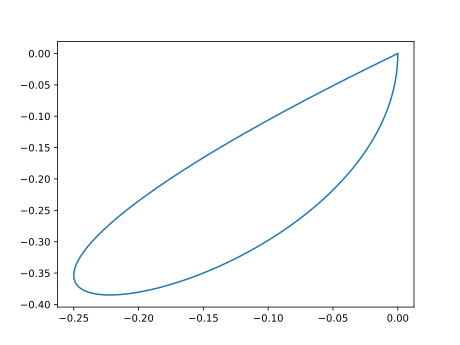
\includegraphics[height=5cm]{figures/discontinuous_curve.pdf}
	\caption{Discontinuous curve where the components are governed by continuous polynomials.}
	\label{fig:disc}
\end{figure}


\newpage

\subsection{Does the Chord Length Always Converge?}

Denote $\{(x(\frac{k}{N}), y(\frac{k}{N}))|k=0,...,N\}$ as a uniform sampling of a 2D curve
$c(t) = (x(t), y(t)), t \in \big[0,1\big]$. As the number of sampling N increases, does chord length monotonically
increase (non-decrease) ? No. \\
Counterexample: consider the equation below, which is shown in Figure~\ref{fig:abs}

\begin{equation}
c(t):=(2t-1, |2t-1|),\, t	\in \big[0,1\big]
\end{equation}

\begin{figure}[h]
	\centering
	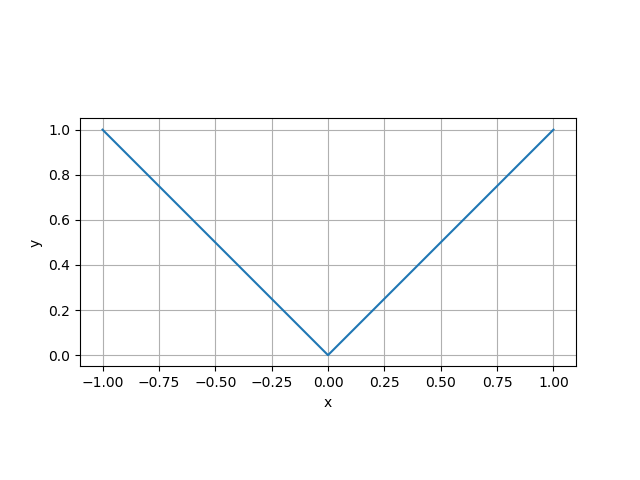
\includegraphics[height=5cm]{figures/plot_abs_function.pdf}
	\caption{Image of $c(t)$}
	\label{fig:abs}
\end{figure}

Now we sample the curve with two different amounts of samples in Figure~\ref{fig:sampled_abs} and observe
\begin{itemize}
	\item $N=3$: the chord length is $2\sqrt{2}$
	\item $N=4$: the chord length is $1 + \sqrt{2}$
\end{itemize}
So we increased N, but the chord length decreased. The counterexample is complete.

\begin{figure}[h]
	\begin{subfigure}{0.49\textwidth}
	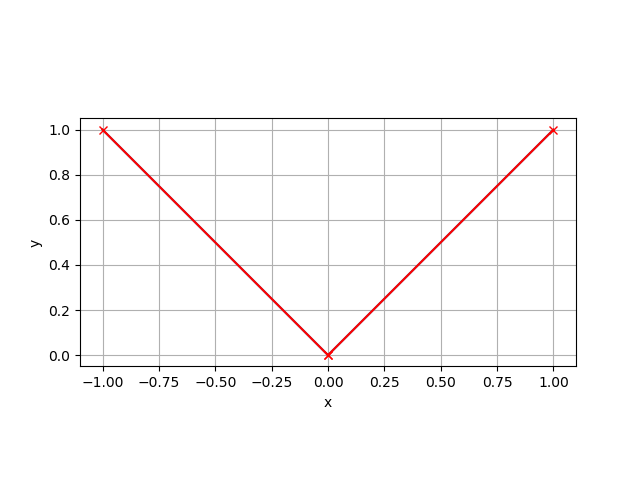
\includegraphics[width=\textwidth]{figures/plot_abs_function_n3.pdf}
	\subcaption{$N=3$}
	\end{subfigure}
	\begin{subfigure}{0.49\textwidth}
	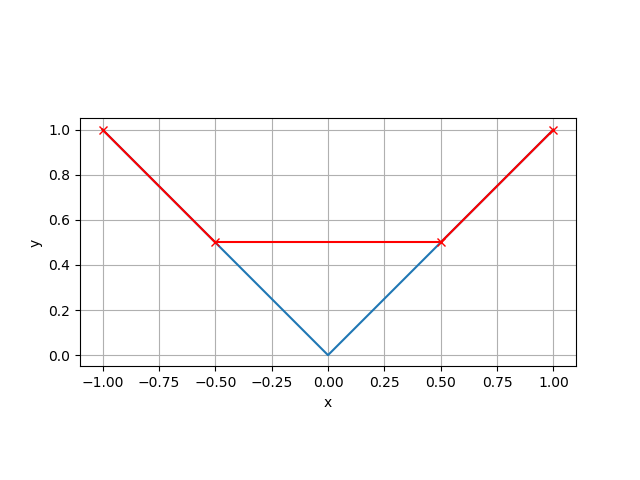
\includegraphics[width=\textwidth]{figures/plot_abs_function_n4.pdf}
	\subcaption{$N=4$}
	\end{subfigure}
	\caption{Uniformly sampled chords for different amounts $N$.}\label{fig:sampled_abs}
\end{figure}
\subsection{A Sequence of 2D Curves}
	
\end{document}
